\documentclass[12pt,a4paper]{article}
\usepackage[top=1in, bottom=1in, left=1.25in, right=1in]{geometry}
\usepackage{graphicx}
\usepackage{array}
\usepackage{setspace}
\usepackage{tabularx}
\usepackage{float}
\usepackage{enumitem}
\usepackage{caption}
\usepackage{amsmath}
\usepackage{sectsty}
\usepackage{titlesec}
\usepackage{fancyhdr}
\usepackage{ragged2e}
\usepackage{fontspec}
\setmainfont{Times New Roman}
\pagestyle{fancy}
\fancyhf{}
\fancyfoot[C]{\thepage}
\renewcommand{\headrulewidth}{0pt}
\fancypagestyle{plain}{%
  \fancyhf{}
  \fancyfoot[C]{\thepage}
  \renewcommand{\headrulewidth}{0pt}
}

\newcolumntype{C}[1]{>{\centering\arraybackslash}p{#1}}
\newcolumntype{Z}{>{\raggedright\arraybackslash}X}

\setlength{\parindent}{1.5em}
\setlength{\parskip}{0pt}
\onehalfspacing

\sectionfont{\fontsize{16}{19}\selectfont\bfseries}
\subsectionfont{\fontsize{14}{17}\selectfont\bfseries}
\subsubsectionfont{\fontsize{12}{14}\selectfont\bfseries\itshape}

\captionsetup{labelsep=space, font={bf,small}, skip=4pt}

\begin{document}

% ============================================================
%                     COVER PAGE
% ============================================================
\begin{titlepage}
\centering
\setstretch{1.2}

\vspace*{0.6cm}
{\fontsize{22}{26}\selectfont\textbf{PATAN MULTIPLE CAMPUS}}\par
\vspace{0.2cm}
{\fontsize{16}{20}\selectfont\textbf{PATAN DHOKA, LALITPUR}}\par
\vspace{0.1cm}
{\fontsize{12}{15}\selectfont (Department of Computer Science and Information Technology)}\par

\vspace{1.2cm}

\includegraphics[width=4.5cm]{logo_tu.jpeg}\par
\vspace{1.2cm}

{\fontsize{14}{18}\selectfont\textbf{SOFTWARE PROJECT MANAGEMENT}}\par
\vspace{0.3cm}
{\fontsize{22}{26}\selectfont\textbf{LAB REPORT}}\par

\vfill

\noindent
\begin{minipage}[t]{0.48\textwidth}
\underline{\textbf{Submitted By:}}\\[0.15cm]
Name: \textbf{Samir Paudel}\\
Program: BSc. CSIT\\
Semester: 7th Semester\\
Section: D\\
Roll No: 114/079\\
Symbol No: \textbf{79010103}
\end{minipage}
\hfill
\begin{minipage}[t]{0.48\textwidth}
\begin{flushleft}
\underline{\textbf{Submitted To:}}\\[0.15cm]
Department of Computer Science and\\
Information Technology\\
Patan Multiple Campus\\
Patan Dhoka, Lalitpur\\
Tribhuvan University
\end{flushleft}
\end{minipage}

\vspace{1.5cm}

\end{titlepage}

\newgeometry{top=1in, bottom=1in, left=0.8in, right=0.8in}
\justifying

% ============================================================
%                     INDEX
% ============================================================
\newpage
\pagenumbering{roman}
\setcounter{page}{1}

\begin{center}
    \vspace*{0.3cm}
    {\fontsize{20}{24}\selectfont\textbf{INDEX}}
    \vspace{0.5cm}
\end{center}

\renewcommand{\arraystretch}{1.8}
\noindent\begin{tabularx}{\textwidth}{|C{0.8cm}|Z|C{2.5cm}|C{2.5cm}|}
\hline
\textbf{S.N.} & \centering\textbf{Lab Task} & \textbf{Date} & \textbf{Signature} \\ \hline
1 & \textbf{Student Profile Management System - Project Scheduling} \newline
   Consider the Student Profile Management project details with different
   activities, durations, predecessors, and resources. Create the project
   in ProjectLibre, build the WBS and RBS, generate both basic and
   relationship-based Gantt charts, produce Task Usage and Resource Usage
   reports, and draw the PERT/CPM network diagram. Identify the critical
   path and determine the project duration. & July 8, 2026 & \\ \hline
2 & \textbf{PERT Diagram and Critical Path} \newline
   Given a set of project activities with predecessors and durations,
   draw the PERT network diagram. Perform forward pass (ES, EF) and
   backward pass (LS, LF) computations, calculate slack for each
   activity, and determine the critical path and total project duration. & July 8, 2026 & \\ \hline
3 & \textbf{AOA Network Diagram and Critical Path Calculation} \newline
   Given a set of activities in Activity-on-Arrow (AOA) notation with
   node pairs and durations, compute earliest and latest event times
   (TE and TL), identify critical nodes and activities, and determine
   the critical path and total project duration. & July 8, 2026 & \\ \hline
\end{tabularx}

\vfill
\begin{center}
    \textit{Department of Computer Science and Information Technology}
\end{center}

% ============================================================
%                     OBJECTIVE
% ============================================================
\newpage
\section*{Objective}

The objective of this lab is to understand the fundamentals of project scheduling
and network modeling used in software project management. Specifically, this lab
covers:

\begin{enumerate}[leftmargin=*, itemsep=4pt]
    \item To \textbf{create a project schedule} using project management software
          (MS~Project / OpenProj / ProjectLibre).
    \item To \textbf{construct a WBS and RBS} - Work Breakdown Structure and
          Resource Breakdown Structure for the Student Profile Management project.
    \item To \textbf{generate Gantt charts} - both basic and relationship-based
          (with dependency arrows).
    \item To \textbf{produce reports} - Task Usage and Resource Usage reports
          with resource allocation details.
    \item To \textbf{draw PERT/CPM diagrams} - identifying the critical path
          and computing floats for project network analysis.
\end{enumerate}

% ============================================================
%                     TASK 1
% ============================================================
\newpage
\pagenumbering{arabic}
\setcounter{page}{1}
\section*{Task 1: Student Profile Management System - Project Scheduling}

\subsection*{Overview}

This task involves creating a complete project schedule for a \textit{Student
Profile Management System} using ProjectLibre, an open-source alternative to
Microsoft Project. The exercise covers project initialization, work breakdown
structure (WBS) creation, Gantt chart generation, resource allocation, and
network analysis.

\subsection*{Project Initialization}

The project was created in ProjectLibre by selecting \textbf{File $\to$ New}
and entering the following parameters:

\begin{itemize}[leftmargin=*, itemsep=4pt]
    \item \textbf{Project Name:} Student Profile Management
    \item \textbf{Start Date:} 20/02/2024
    \item \textbf{Manager:} Samir Paudel
    \item \textbf{Organization:} Patan Multiple Campus
\end{itemize}

The project calendar was set to \textbf{Standard} with 8 working hours per day.

\begin{figure}[h!]
\centering
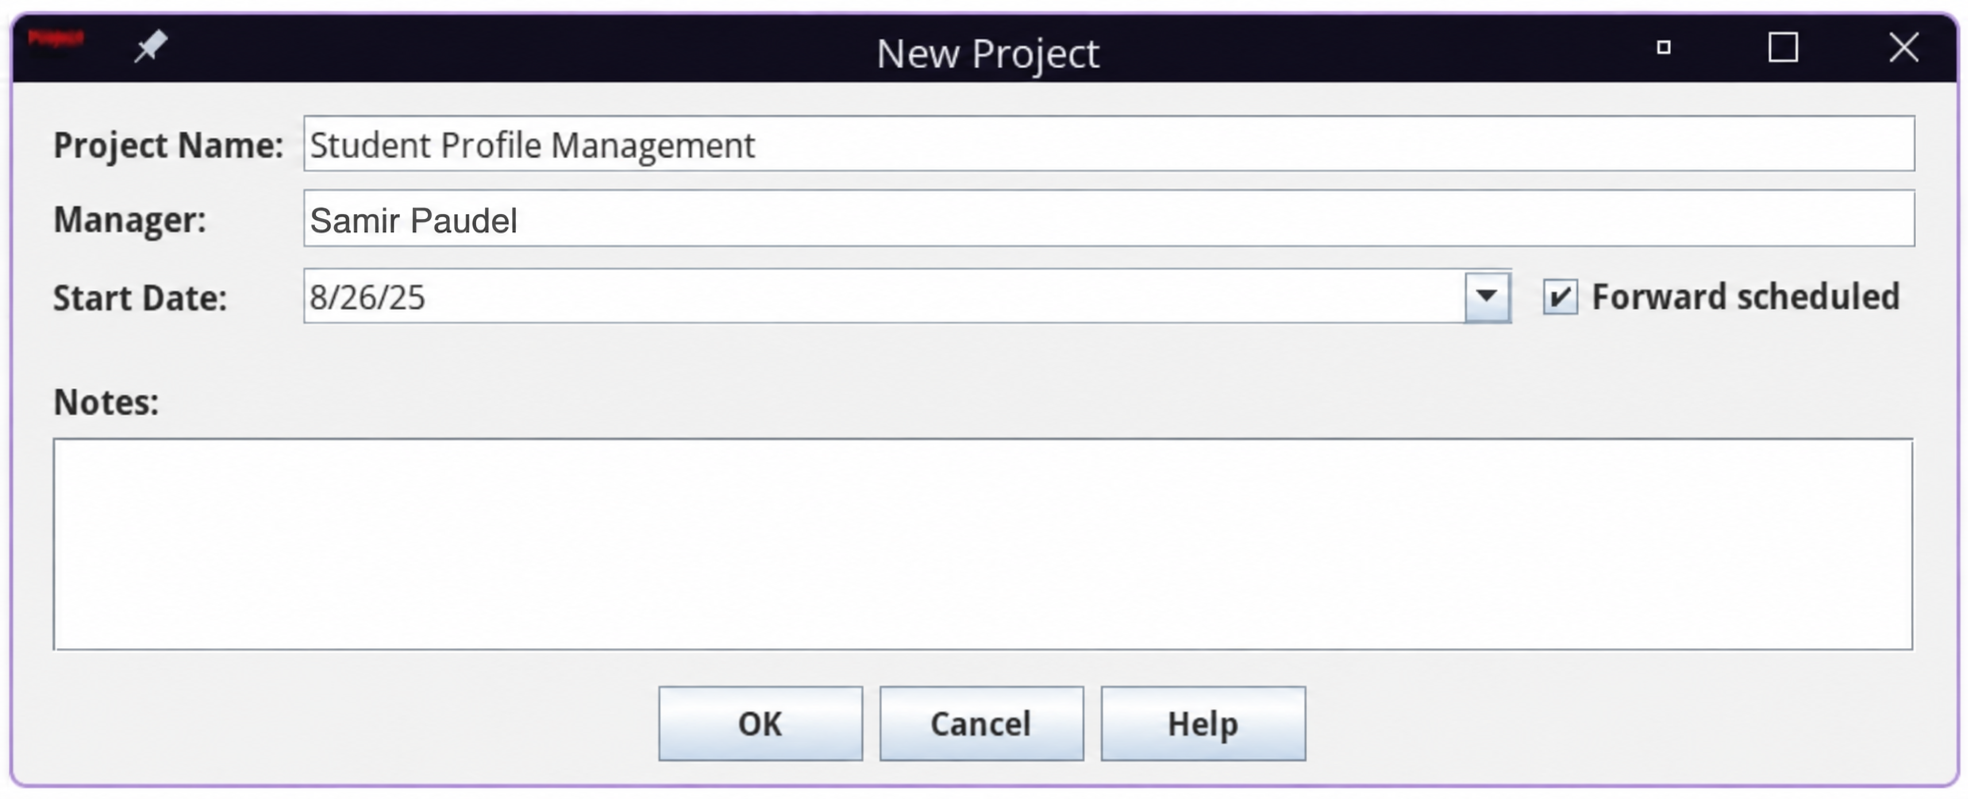
\includegraphics[width=0.7\textwidth]{images/0_project_dialog.png}
\caption{New Project dialog with \textit{Student Profile Management}}
\end{figure}

\subsection*{Work Breakdown Structure}

The project was decomposed into six sequential activities. Each activity was
assigned a duration, start date, predecessor(s), and resource allocation as
listed in Table~\ref{tab:wbs}.

\begin{table}[h!]
\centering
\renewcommand{\arraystretch}{1.0}
\footnotesize
\renewcommand{\tabcolsep}{2.5pt}
\begin{tabular}{|c|l|c|c|c|c|l|}
\hline
\textbf{S.N.} & \textbf{Activity} & \textbf{Dur.} & \textbf{Start} & \textbf{Finish} & \textbf{Pre.} & \textbf{Resource} \\ \hline
1 & Planning \& Analysis & 7 & 2024-02-20 & 2024-02-26 & - & Team Leader (100\%) \\ \hline
2 & Requirement Collection \& Definition & 15 & 2024-02-27 & 2024-03-12 & 1 & System Analyst (20\%) \\ \hline
3 & Designing & 7 & 2024-03-13 & 2024-03-19 & 2 & Designer (15\%) \\ \hline
4 & Development & 21 & 2024-03-20 & 2024-04-09 & 2, 3 & Programmer (70\%) \\ \hline
5 & Testing & 8 & 2024-04-10 & 2024-04-17 & 2, 3, 4 & Test Engineer (20\%) \\ \hline
6 & Deployment & 7 & 2024-04-18 & 2024-04-24 & 3, 4, 5 & - \\ \hline
\end{tabular}
\caption{WBS Data Table as entered in ProjectLibre}
\label{tab:wbs}
\end{table}

All dependencies were set to Finish-to-Start (FS), meaning each successor task
begins the day after the latest-finishing predecessor completes. The total
project duration spans 65 calendar days, from 20 February 2024 to 24 April 2024.

\subsection*{Gantt Chart Visualization}

With all tasks, durations, and dependencies entered, ProjectLibre automatically
renders the Gantt chart for the project schedule.

\begin{figure}[h!]
\centering
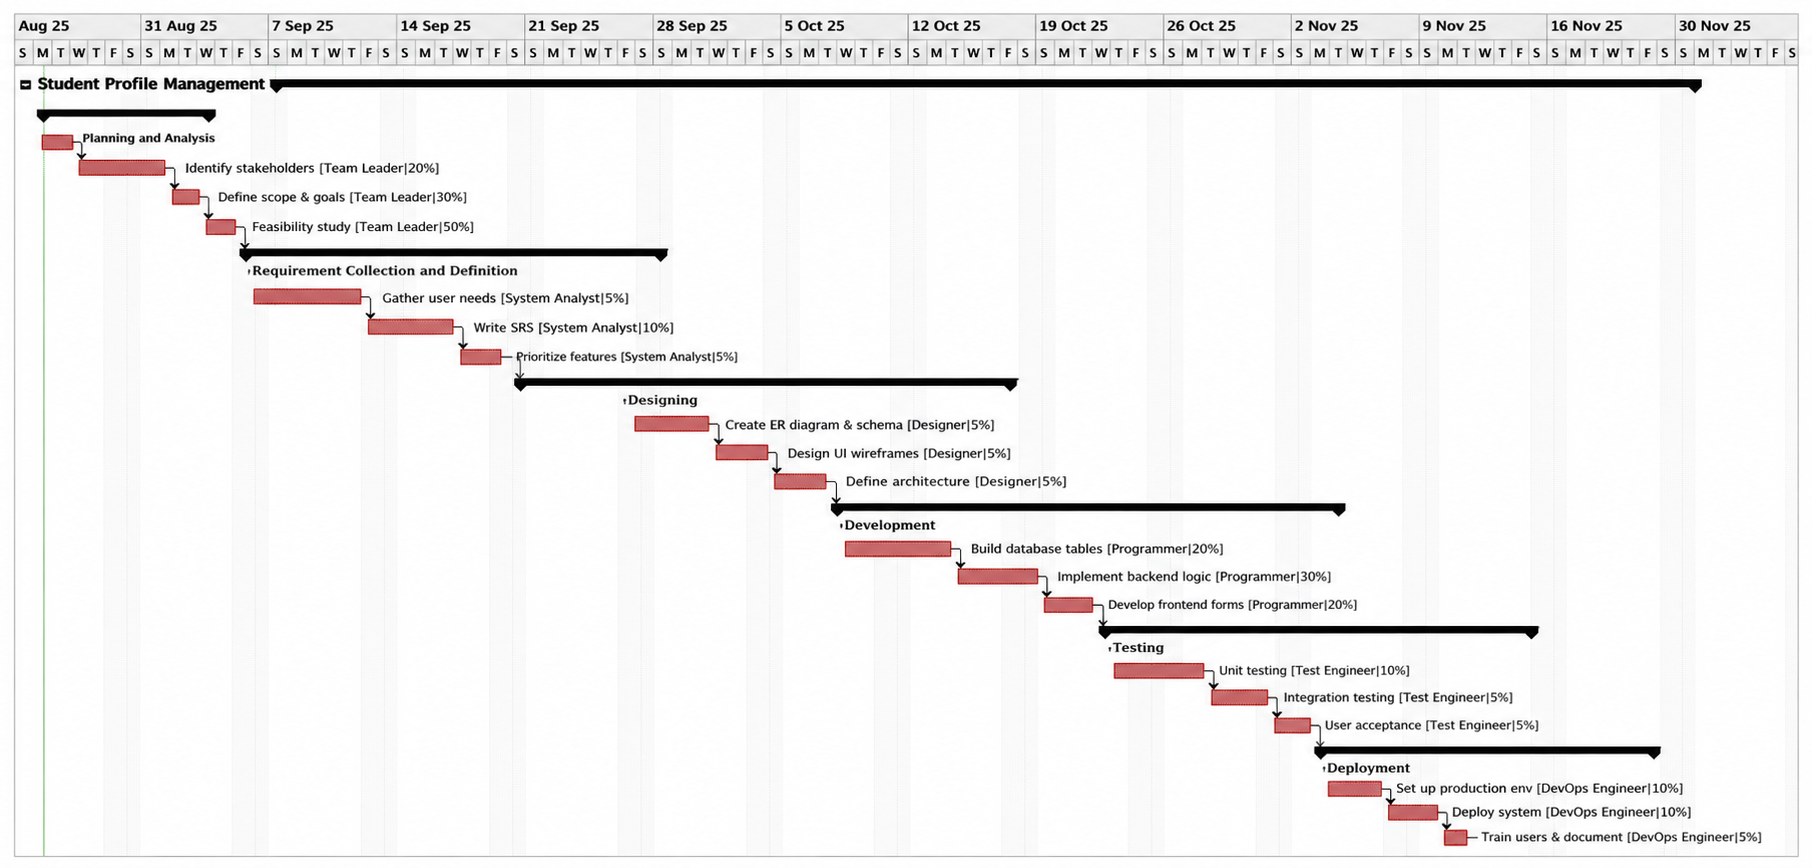
\includegraphics[width=0.85\textwidth]{images/2_overall_gantt_chart.png}
\caption{Gantt Chart - Student Profile Management System}
\end{figure}

\subsection*{WBS and RBS Diagrams}

The \textit{Work Breakdown Structure} decomposes the project into six
hierarchical phases, each representing a distinct deliverable. The
\textit{Resource Breakdown Structure} categorizes resources by type-in
this case, all human resources assigned to the project.

\begin{figure}[H]
\centering
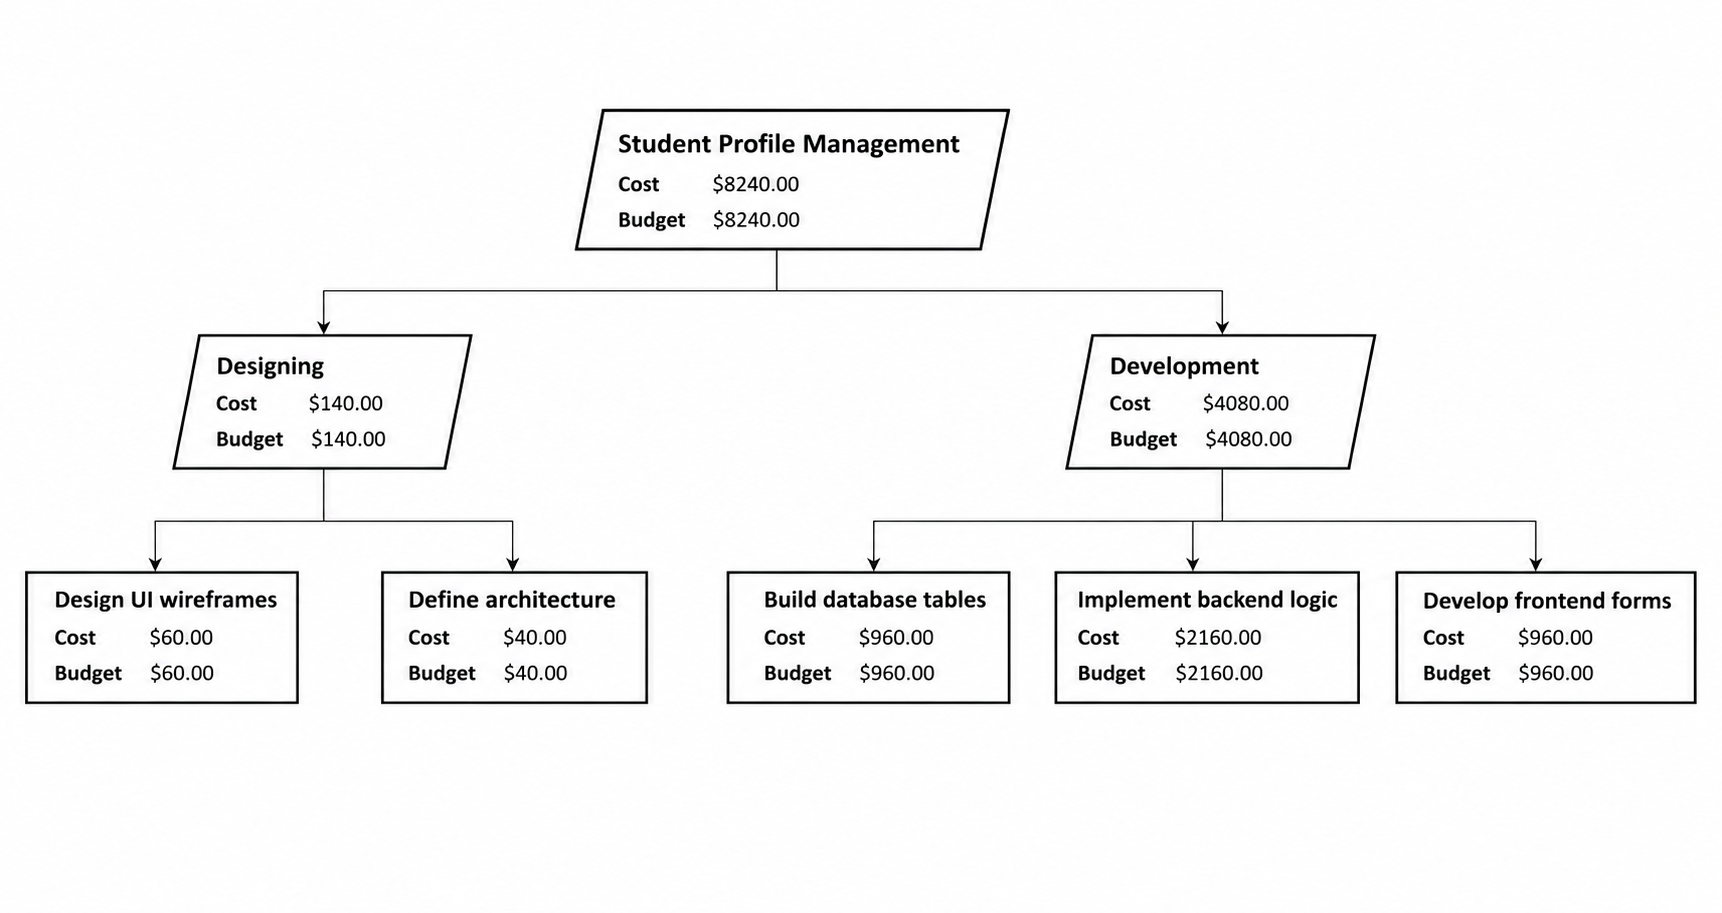
\includegraphics[width=0.85\textwidth]{images/3_WBS.png}
\caption{Work Breakdown Structure - Student Profile Management System}
\end{figure}

\begin{figure}[H]
\centering
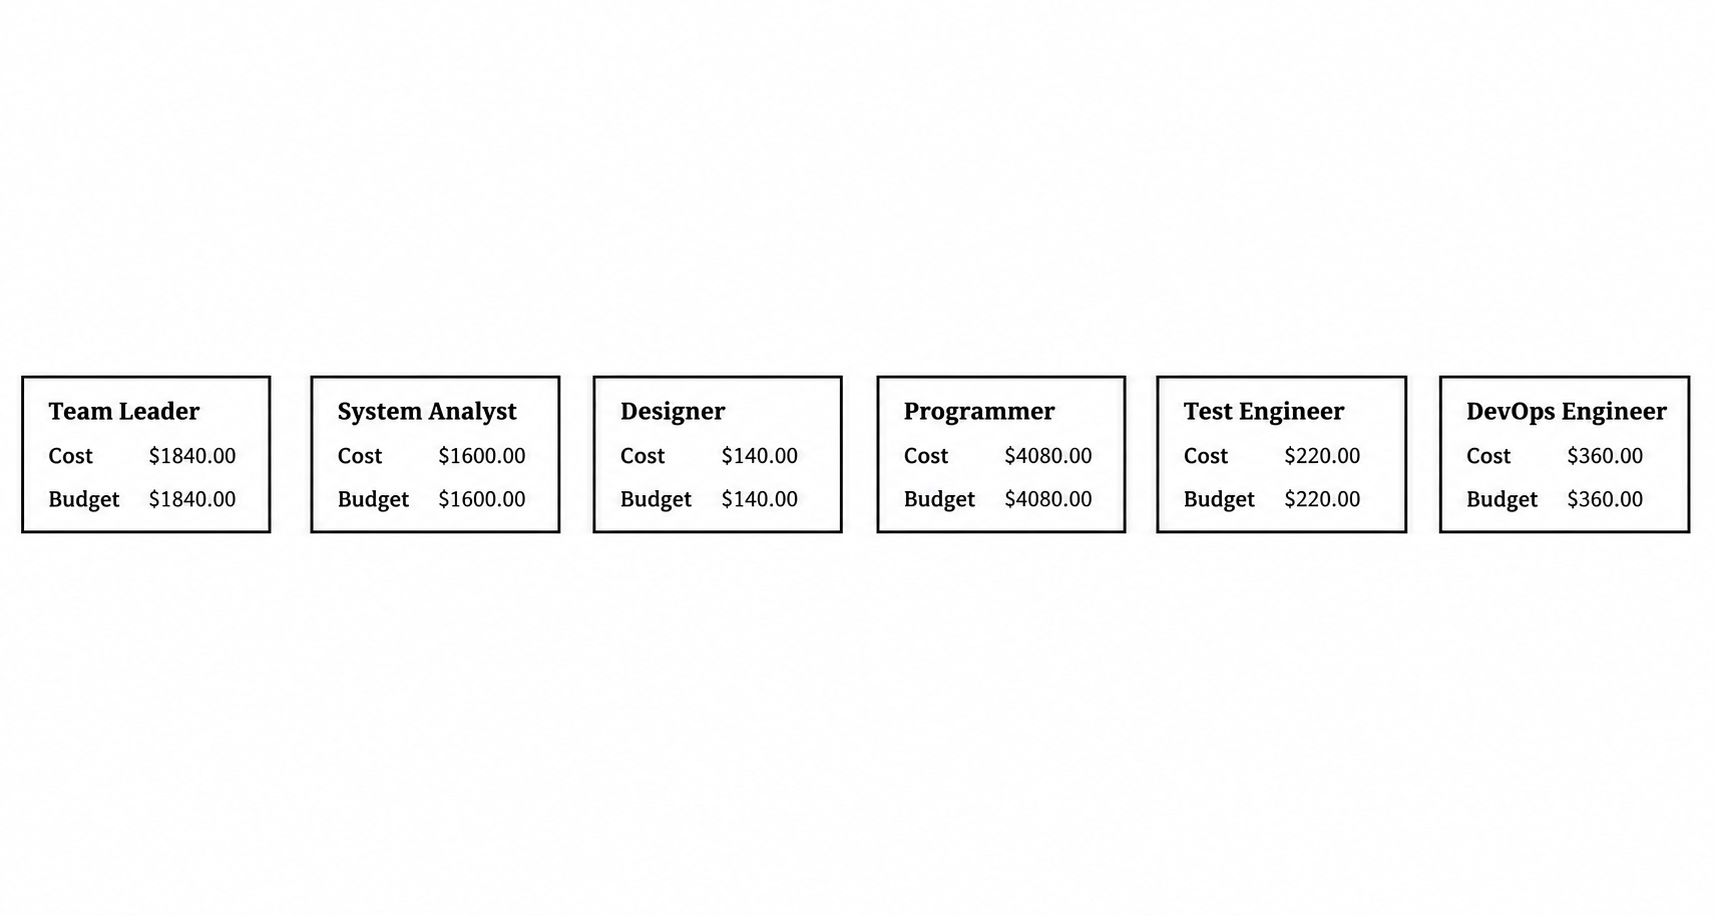
\includegraphics[width=0.7\textwidth]{images/4_rbs.png}
\caption{Resource Breakdown Structure - Student Profile Management System}
\end{figure}

\subsection*{Task Usage and Resource Usage Reports}

Task usage and resource usage reports quantify the effort distribution.
Effort is calculated as:

\[
\text{Work} = \text{Duration} \times \text{Resource Units}
\]

For example, the Programmer assigned at 70\% for 21 days yields
$21 \times 8 \times 0.70 = 117.6$ hours.

\begin{table}[h!]
\centering
\renewcommand{\arraystretch}{1.15}
\footnotesize
\renewcommand{\tabcolsep}{4pt}
\begin{tabular}{|c|l|c|c|c|c|}
\hline
\textbf{S.N.} & \textbf{Task} & \textbf{Du.} & \textbf{Resource} & \textbf{Units} & \textbf{Work (hrs)} \\ \hline
1 & Planning \& Analysis & 7d & Team Leader & 100\% & 56.0 \\ \hline
2 & Requirement Collection \& Definition & 15d & System Analyst & 20\% & 24.0 \\ \hline
3 & Designing & 7d & Designer & 15\% & 8.4 \\ \hline
4 & Development & 21d & Programmer & 70\% & 117.6 \\ \hline
5 & Testing & 8d & Test Engineer & 20\% & 12.8 \\ \hline
6 & Deployment & 7d & Not assigned & - & 0.0 \\ \hline
\end{tabular}
\caption{Task Usage Report}
\end{table}

\begin{table}[h!]
\centering
\renewcommand{\arraystretch}{1.15}
\footnotesize
\renewcommand{\tabcolsep}{4pt}
\begin{tabular}{|c|l|c|c|}
\hline
\textbf{S.N.} & \textbf{Resource} & \textbf{Assigned Task(s)} & \textbf{Total Work (hrs)} \\ \hline
1 & Team Leader & Planning \& Analysis & 56.0 \\ \hline
2 & System Analyst & Requirement Collection \& Definition & 24.0 \\ \hline
3 & Designer & Designing & 8.4 \\ \hline
4 & Programmer & Development & 117.6 \\ \hline
5 & Test Engineer & Testing & 12.8 \\ \hline
\end{tabular}
\caption{Resource Usage Report}
\end{table}

\subsection*{Network Modeling - PERT Chart and CPM}

The PERT/CPM network diagram was generated using ProjectLibre's
\textbf{View $\to$ Network Diagram} option. Each node displays the task ID,
name, duration, and the computed Early Start (ES), Early Finish (EF), Late
Start (LS), and Late Finish (LF). Critical tasks-those with zero
slack-are highlighted in red.

\begin{figure}[h!]
\centering
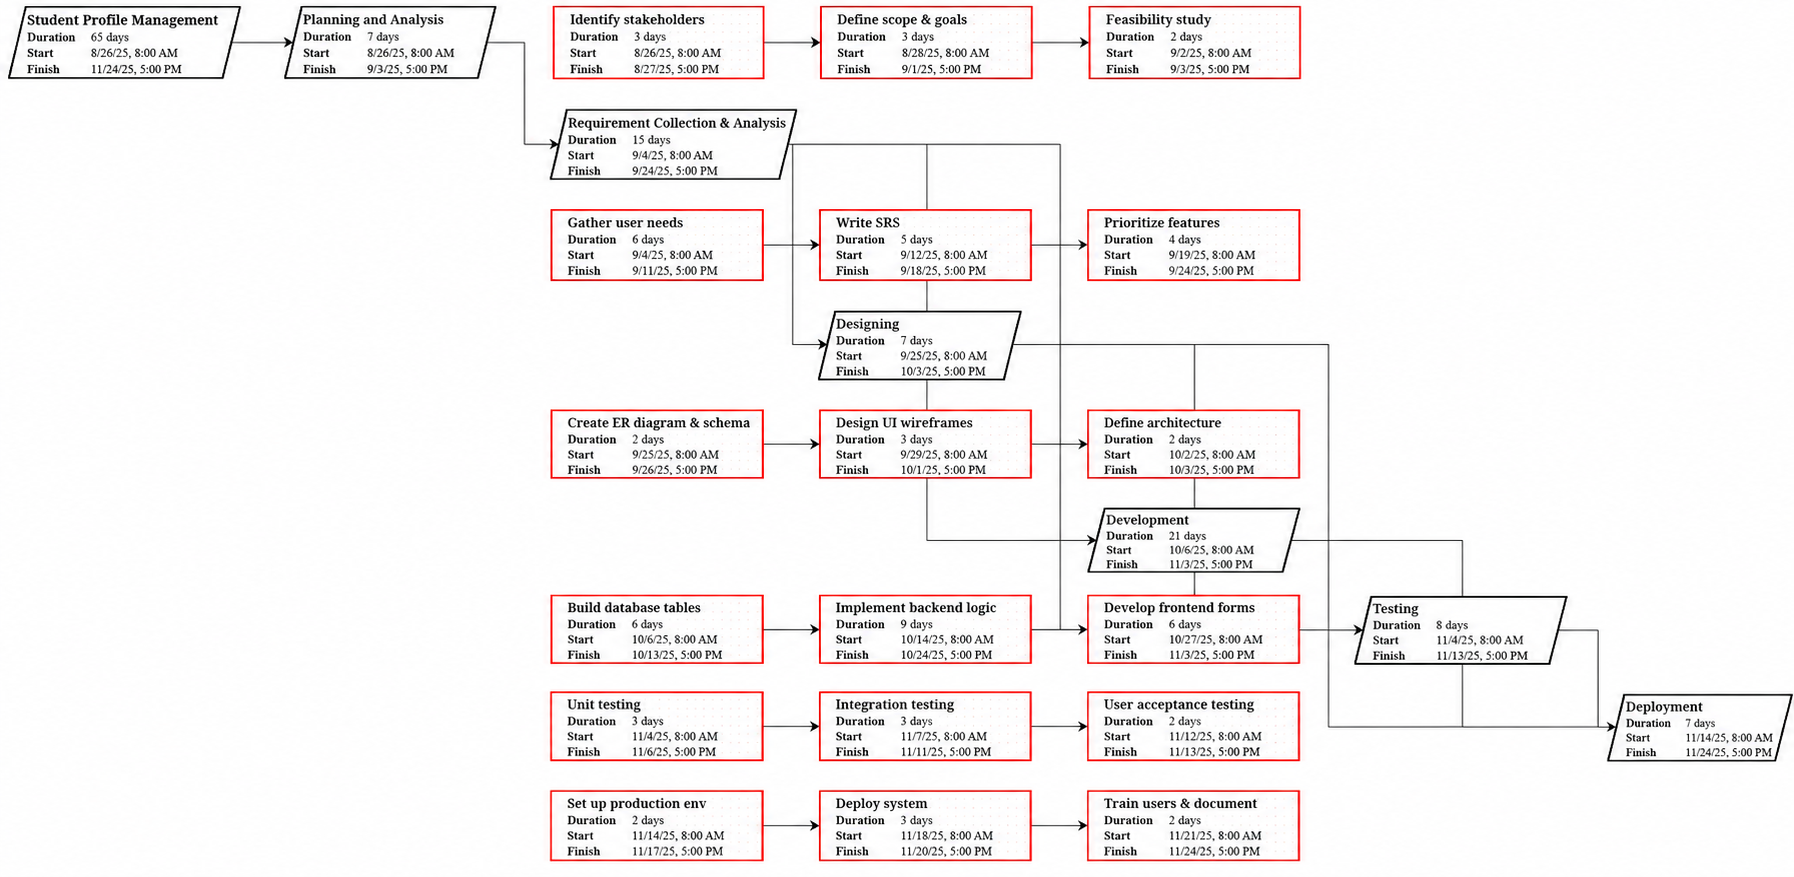
\includegraphics[width=0.85\textwidth]{images/5_pert_cpm_diagram.png}
\caption{PERT/CPM Network Diagram (AON) - Student Profile Management System}
\end{figure}

\subsubsection*{Analysis}

Since every activity depends on the completion of all its predecessors in a
purely sequential chain ($1 \to 2 \to 3 \to 4 \to 5 \to 6$), there exists only
one path through the network. Consequently, all six activities are critical
with zero slack.

\begin{center}
\renewcommand{\arraystretch}{1.3}
\begin{tabular}{|c|c|}
\hline
\textbf{Metric} & \textbf{Result} \\ \hline
Critical Path & $1 \to 2 \to 3 \to 4 \to 5 \to 6$ \\ \hline
Project Duration & $7 + 15 + 7 + 21 + 8 + 7 = \textbf{65 days}$ \\ \hline
\end{tabular}
\end{center}

% ============================================================
%                     TASK 2
% ============================================================
\newpage
\section*{Task 2: PERT Diagram and Critical Path}

\subsection*{Problem Definition}

A project consists of six activities with the precedence relationships and
durations given in Table~\ref{tab:pert-activities}.

\begin{table}[h!]
\centering
\renewcommand{\arraystretch}{1.25}
\begin{tabular}{|c|c|c|}
\hline
\textbf{Activity} & \textbf{Predecessor(s)} & \textbf{Duration (days)} \\ \hline
A & - & 2 \\ \hline
B & A & 4 \\ \hline
C & A & 5 \\ \hline
D & B & 6 \\ \hline
E & C & 3 \\ \hline
F & D, E & 4 \\ \hline
\end{tabular}
\caption{Activities with Predecessors and Durations}
\label{tab:pert-activities}
\end{table}

\subsection*{Forward Pass}

The forward pass computes the Earliest Start (ES) and Earliest Finish (EF)
times for each activity:

\[
\begin{aligned}
\text{ES(A)} &= 0, \quad \text{EF(A)} = 0 + 2 = 2 \\
\text{ES(B)} &= \text{EF(A)} = 2, \quad \text{EF(B)} = 2 + 4 = 6 \\
\text{ES(C)} &= \text{EF(A)} = 2, \quad \text{EF(C)} = 2 + 5 = 7 \\
\text{ES(D)} &= \text{EF(B)} = 6, \quad \text{EF(D)} = 6 + 6 = 12 \\
\text{ES(E)} &= \text{EF(C)} = 7, \quad \text{EF(E)} = 7 + 3 = 10 \\
\text{ES(F)} &= \max(\text{EF(D)}, \text{EF(E)}) = \max(12, 10) = 12, \quad \text{EF(F)} = 12 + 4 = 16
\end{aligned}
\]

\subsection*{Backward Pass}

The backward pass computes the Latest Finish (LF) and Latest Start (LS) times:

\[
\begin{aligned}
\text{LF(F)} &= 16, \quad \text{LS(F)} = 16 - 4 = 12 \\
\text{LF(D)} &= \text{LS(F)} = 12, \quad \text{LS(D)} = 12 - 6 = 6 \\
\text{LF(E)} &= \text{LS(F)} = 12, \quad \text{LS(E)} = 12 - 3 = 9 \\
\text{LF(B)} &= \text{LS(D)} = 6, \quad \text{LS(B)} = 6 - 4 = 2 \\
\text{LF(C)} &= \text{LS(E)} = 9, \quad \text{LS(C)} = 9 - 5 = 4 \\
\text{LF(A)} &= \min(\text{LS(B)}, \text{LS(C)}) = \min(2, 4) = 2, \quad \text{LS(A)} = 2 - 2 = 0
\end{aligned}
\]

\subsection*{Slack Computation and Critical Path}

Slack is calculated as $\text{Slack} = \text{LS} - \text{ES}$. Activities with
zero slack lie on the critical path.

\begin{table}[h!]
\centering
\renewcommand{\arraystretch}{1.25}
\footnotesize
\renewcommand{\tabcolsep}{4pt}
\begin{tabular}{|c|c|c|c|c|c|c|}
\hline
\textbf{Activity} & \textbf{ES} & \textbf{EF} & \textbf{LS} & \textbf{LF} & \textbf{Slack} & \textbf{Critical} \\ \hline
A & 0 & 2 & 0 & 2 & 0 & Yes \\ \hline
B & 2 & 6 & 2 & 6 & 0 & Yes \\ \hline
C & 2 & 7 & 4 & 9 & 2 & No \\ \hline
D & 6 & 12 & 6 & 12 & 0 & Yes \\ \hline
E & 7 & 10 & 9 & 12 & 2 & No \\ \hline
F & 12 & 16 & 12 & 16 & 0 & Yes \\ \hline
\end{tabular}
\caption{Slack / Float Analysis}
\end{table}

\begin{figure}[h!]
\centering
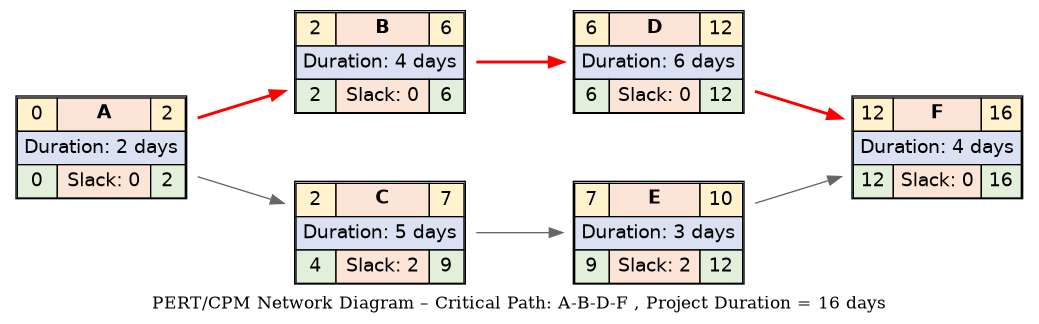
\includegraphics[width=0.7\textwidth]{images/6_pert_nw_diagram.png}
\caption{PERT Network Diagram - Activities A to F}
\end{figure}

\subsection*{Path Comparison}

Two paths emerge from the network:

\[
\begin{aligned}
\text{Path A--B--D--F} &= 2 + 4 + 6 + 4 = 16 \text{ days} \\
\text{Path A--C--E--F} &= 2 + 5 + 3 + 4 = 14 \text{ days}
\end{aligned}
\]

The critical path is the longest path through the network.

\begin{center}
\renewcommand{\arraystretch}{1.3}
\begin{tabular}{|c|c|}
\hline
\textbf{Metric} & \textbf{Result} \\ \hline
Critical Path & A $\to$ B $\to$ D $\to$ F \\ \hline
Project Duration & \textbf{16 days} \\ \hline
\end{tabular}
\end{center}

% ============================================================
%                     TASK 3
% ============================================================
\newpage
\section*{Task 3: AOA Network Diagram and Critical Path Calculation}

\subsection*{Problem Definition}

A project is represented using Activity-on-Arrow (AOA) notation, where each
activity is defined by its start and end node indices $(i, j)$ with
associated durations, as shown in Table~\ref{tab:aoa}.

\begin{table}[h!]
\centering
\renewcommand{\arraystretch}{1.25}
\begin{tabular}{|c|c|}
\hline
\textbf{Activity (i, j)} & \textbf{Duration (Days)} \\ \hline
(1, 2) & 4 \\ \hline
(1, 3) & 6 \\ \hline
(2, 4) & 5 \\ \hline
(3, 4) & 3 \\ \hline
(4, 5) & 2 \\ \hline
(3, 5) & 8 \\ \hline
\end{tabular}
\caption{Project activities in AOA notation}
\label{tab:aoa}
\end{table}

\subsection*{Forward Pass - Earliest Event Times}

The earliest event time $E(j)$ for each node is computed starting from node 1:

\[
\begin{aligned}
E(1) &= 0 \\
E(2) &= E(1) + 4 = 4 \\
E(3) &= E(1) + 6 = 6 \\
E(4) &= \max[E(2) + 5,\; E(3) + 3] = \max[9, 9] = 9 \\
E(5) &= \max[E(4) + 2,\; E(3) + 8] = \max[11, 14] = 14
\end{aligned}
\]

\subsection*{Backward Pass - Latest Event Times}

The latest event time $L(i)$ for each node is computed backward from node 5:

\[
\begin{aligned}
L(5) &= 14 \\
L(4) &= L(5) - 2 = 12 \\
L(3) &= \min[L(4) - 3,\; L(5) - 8] = \min[9, 6] = 6 \\
L(2) &= L(4) - 5 = 7 \\
L(1) &= \min[L(2) - 4,\; L(3) - 6] = \min[3, 0] = 0
\end{aligned}
\]

\subsection*{Event Time Table}

\begin{table}[h!]
\centering
\renewcommand{\arraystretch}{1.25}
\begin{tabular}{|c|c|c|c|c|}
\hline
\textbf{Node} & \textbf{Earliest $E$} & \textbf{Latest $L$} & \textbf{Slack} & \textbf{Critical} \\ \hline
1 & 0 & 0 & 0 & Yes \\ \hline
2 & 4 & 7 & 3 & No \\ \hline
3 & 6 & 6 & 0 & Yes \\ \hline
4 & 9 & 12 & 3 & No \\ \hline
5 & 14 & 14 & 0 & Yes \\ \hline
\end{tabular}
\caption{Event time analysis}
\end{table}

\begin{figure}[h!]
\centering
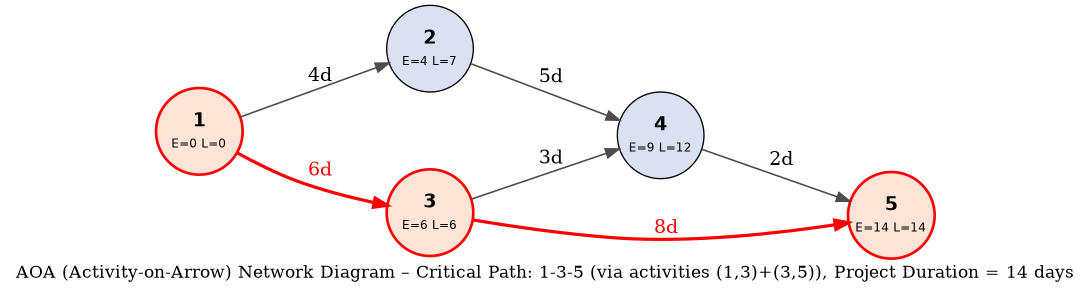
\includegraphics[width=0.7\textwidth]{images/7_AOA_nw_diagram.png}
\caption{AOA Network Diagram - Nodes 1 to 5}
\end{figure}

\subsection*{Critical Path Determination}

An activity $(i, j)$ lies on the critical path if and only if:

\[
E(i) = L(i), \qquad E(j) = L(j), \qquad E(i) + d_{ij} = E(j)
\]

Applying this condition:

\[
\begin{aligned}
(1,3):&\quad E(1)+6 = 6 = E(3), \text{ both nodes critical} \;\to\; \textbf{Critical} \\
(3,5):&\quad E(3)+8 = 14 = E(5), \text{ both nodes critical} \;\to\; \textbf{Critical} \\
(1,2), (2,4), (3,4), (4,5):&\quad \text{fail the equality test} \;\to\; \text{Not critical}
\end{aligned}
\]

\begin{center}
\renewcommand{\arraystretch}{1.3}
\begin{tabular}{|c|c|}
\hline
\textbf{Metric} & \textbf{Result} \\ \hline
Critical Path & 1 $\to$ 3 $\to$ 5 (via activities (1,3) and (3,5)) \\ \hline
Project Duration & $6 + 8 = \textbf{14 days}$ \\ \hline
\end{tabular}
\end{center}

% ============================================================
%                     CONCLUSION
% ============================================================
\newpage
\section*{Conclusion}

This lab provided hands-on experience in software project scheduling using a
project management tool (ProjectLibre) and manual network analysis. The key
learnings from this lab are summarized below.

\vspace{0.2cm}
\noindent\textbf{Key Learnings}

\begin{itemize}[leftmargin=*, itemsep=6pt]
    \item \textbf{Project Planning} - Creating a project plan with a Work
          Breakdown Structure (WBS) linking tasks, durations, dates,
          dependencies and resources.
    \item \textbf{Gantt Charting} - Visualizing the schedule through basic
          and relationship (dependency-linked) Gantt charts.
    \item \textbf{WBS and RBS} - Decomposing the project into WBS and RBS
          hierarchies for clearer planning and resource allocation.
    \item \textbf{Effort Tracking} - Generating Task Usage and Resource
          Usage reports to track effort distribution.
    \item \textbf{Critical Path Analysis} - Applying the forward and backward
          pass technique of PERT/CPM to compute ES, EF, LS, LF, slack, and
          identify the critical path.
\end{itemize}

\vspace{0.2cm}
\noindent\textbf{Summary of Results}

\begin{center}
\renewcommand{\arraystretch}{1.3}
\begin{tabular}{|c|l|c|}
\hline
\textbf{S.N.} & \textbf{Exercise} & \textbf{Critical Path Duration} \\ \hline
1 & Student Profile Management (ProjectLibre) & \textbf{65 days} \\ \hline
2 & PERT Network Analysis (Activities A--F) & \textbf{16 days} \\ \hline
3 & AOA Network Analysis (Nodes 1--5) & \textbf{14 days} \\ \hline
\end{tabular}
\end{center}

\vspace{0.3cm}

\end{document}